\chapter{Results on the Bundled Demo}

Reproduce every number in this chapter with:

\begin{cli}
qp demo\\
qp walkforward -c configs/demo.yaml
\end{cli}

\section{The demo run}

\texttt{configs/demo.yaml}: 8 synthetic symbols, 2013--2024, \texttt{cross\_sectional\_momentum}
(60-day lookback, 5-day skip), volatility-targeted at 10\%/year, weekly
rebalance, 1\,bp commission + 2\,bp spread + 50\,bp/year borrow.

\begin{table}[h]
\footnotesize
\centering
\begin{tabularx}{\textwidth}{L{4.2cm} X L{4.2cm} X}
\toprule
\thh{Metric} & \thh{Value} & \thh{Metric} & \thh{Value} \\
\midrule
Trading days & 3{,}131 & Hit rate & 50.7\% \\
CAGR & 4.57\% & Skew / kurtosis & 0.08 / 2.87 \\
Annualised vol & 7.73\% & Daily VaR$_{95}$ / CVaR$_{95}$ & $-0.74\%$ / $-1.07\%$ \\
Sharpe & 0.62 & Avg.\ gross / net exposure & 1.34 / $-0.03$ \\
Sortino & 0.92 & Avg.\ daily turnover & 0.10 \\
Max drawdown & $-14.87\%$ & Time in market & 97.8\% \\
Calmar & 0.31 & & \\
\bottomrule
\end{tabularx}
\caption{\texttt{runs/demo/metrics.json}, reproduced exactly by \texttt{qp demo}
(fixed seed). Net exposure near zero confirms the book is running
market-neutral, as \texttt{CrossSectionalMomentum} is designed to.}
\end{table}

\begin{figure}[h]
\centering
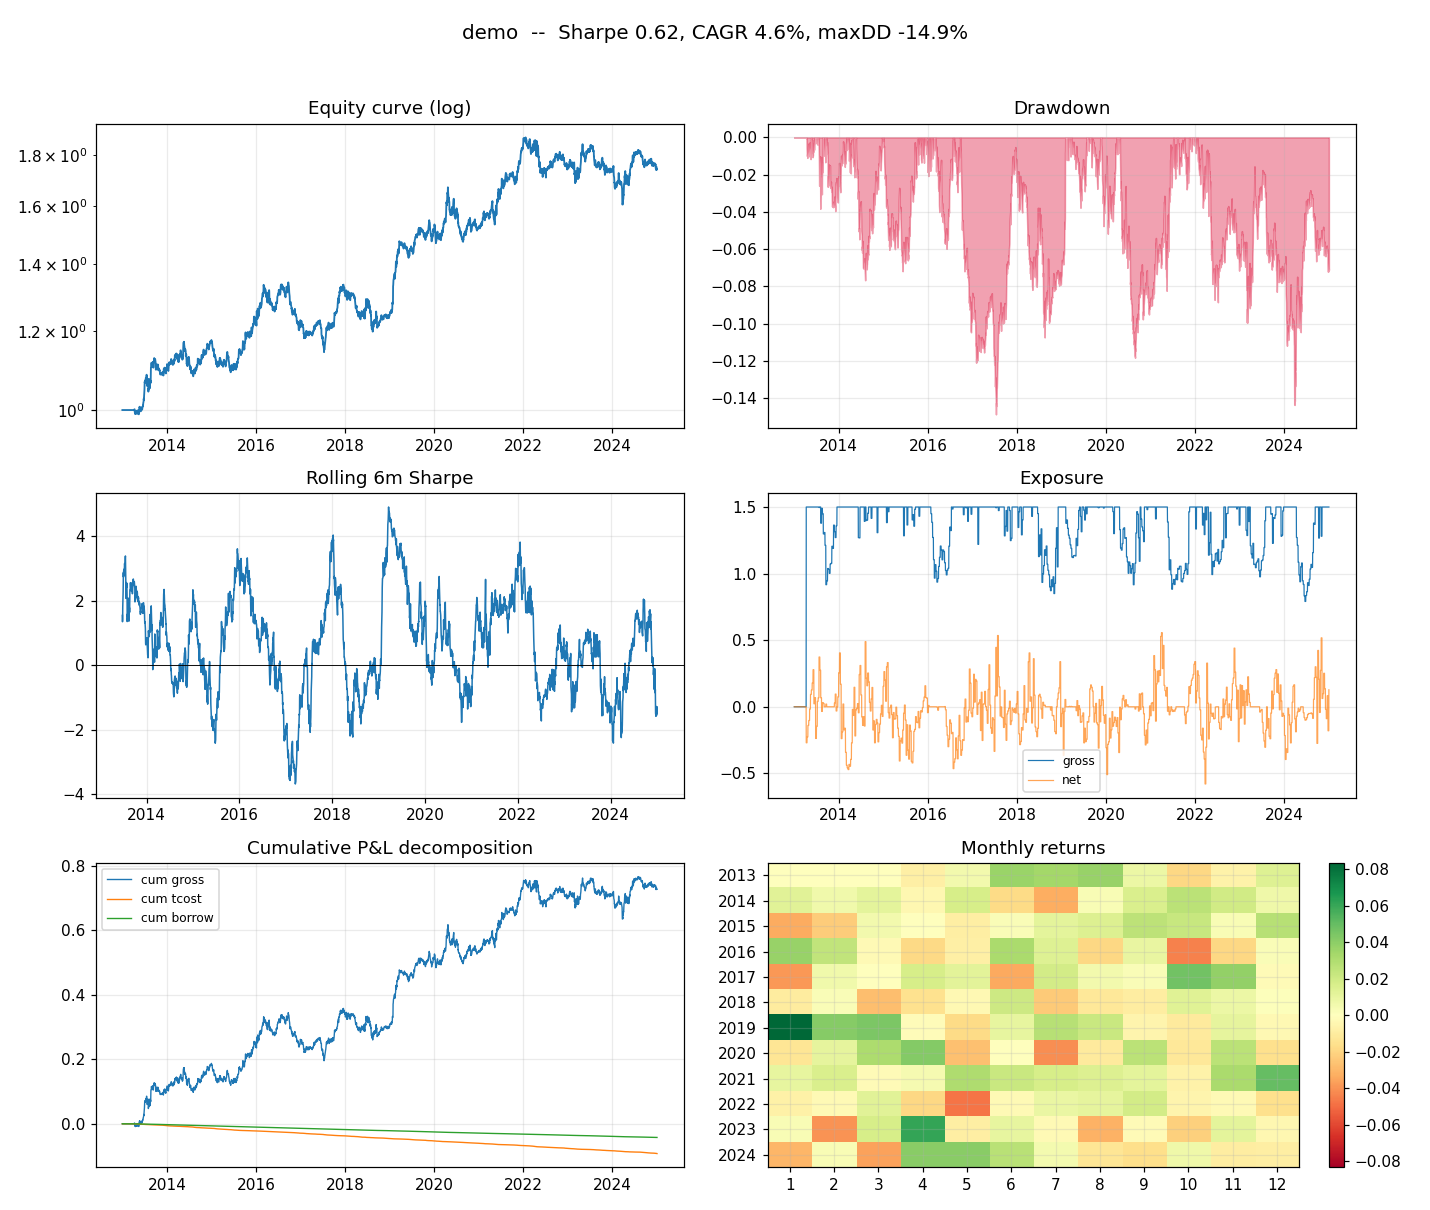
\includegraphics[width=\textwidth]{figures/tearsheet.png}
\caption{\texttt{runs/demo/tearsheet.png}: equity curve, drawdown, rolling
6-month Sharpe, gross/net exposure, cumulative P\&L decomposition (gross vs.\
transaction cost vs.\ borrow cost), and the monthly-return heatmap.}
\end{figure}

\section{Rule versus ML, same data, same costs}

\texttt{qp walkforward} runs \texttt{cross\_sectional\_momentum} and the
walk-forward \texttt{MLSignal} (a \texttt{HistGradientBoostingRegressor} on the
same feature set, 5-day forward-return target) through the identical sizing,
cost, and risk pipeline, on the identical dataset:

\begin{table}[h]
\footnotesize
\centering
\begin{tabularx}{\textwidth}{L{4cm} C{2.2cm} C{2.2cm} C{2.6cm} X}
\toprule
\thh{Variant} & \thh{Sharpe} & \thh{CAGR} & \thh{Max drawdown} & \thh{Avg.\ daily turnover} \\
\midrule
\texttt{cs\_momentum} & \textbf{0.62} & 4.6\% & $-14.9\%$ & 0.10 \\
\texttt{ml\_gbr} & $-0.07$ & $-0.7\%$ & $-21.1\%$ & 0.17 \\
\bottomrule
\end{tabularx}
\caption{Same universe, same walk-forward discipline, same cost model. The
simple rule wins, and by a wide margin.}
\end{table}

A second, independent dataset (\texttt{configs/ml\_walkforward.yaml} --
10 years, 8 different synthetic symbols, a fresh seed) gives the ML signal
Sharpe $-0.57$ on its own -- consistent with the comparison above, not a fluke
of one run.

\section{Why the rule beat the model here}

The synthetic alpha (Chapter~2) is a slow AR(1) process with a $\approx$69-day
half-life. A 60-day trailing-return momentum signal is close to a matched
filter for exactly that process. The ML model is asked to recover the same
signal from a 5-day-ahead target through a gradient-boosted tree over noisy
technical features -- a much harder estimation problem, with far more ways for
the model to fit noise in the training window that does not repeat in the test
window. This is not a defect in the implementation; it is the expected outcome
whenever a flexible model is pointed at a low signal-to-noise, slowly-varying
target without a structural reason to expect it to generalise better than a
simple, correctly-shaped rule. See Chapter~10 for the general version of this
argument and its implications for real markets.
